\documentclass[a4paper]{book}
\usepackage[english]{babel}						% Correct English hyphenation
\usepackage[utf8]{inputenc}					    % Allow for non-English letters
\usepackage{graphicx}							% To include graphics
%\usepackage{natbib}								% Correct citations
\usepackage{geometry} 							% Better geometry
%\usepackage[center]					            % For cropping documents
\usepackage[numbers]{natbib}	
\usepackage[parfill]{parskip}
\usepackage{nameref}
\PassOptionsToPackage{hyphens}{url}\usepackage{hyperref}
\usepackage{float}
\restylefloat{table}

% Author
\newcommand{\thesisAuthor}{Christian Rasmussen}
\newcommand{\thesisTitle}{Finding Related Web Pages for Course \mbox{Material} Based on its Content}
\newcommand{\thesisType}{Specialization project}
\newcommand{\thesisDate}{fall 2013}

% PDF info
\hypersetup{pdfauthor={\thesisAuthor}}
\hypersetup{pdftitle={\thesisTitle}}
\hypersetup{pdfsubject={\thesisType}}

% Citation format
%\bibliographystyle{apalike}
%\bibpunct{[}{]}{;}{a}{,}{,}
\bibliographystyle{unsrtnat}

\mathchardef\mhyphen="2D
\newcommand\tf{\mathit{tf}}
\newcommand\df{\mathit{df}}
\newcommand\idf{\mathit{idf}}
\newcommand\tfidf{\mathit{tf\mhyphen idf}}


\begin{document}

\begin{titlepage}

\noindent {\large \textbf{\thesisAuthor}}
\vspace{2cm}

\noindent {\Huge \thesisTitle}
\vspace{2cm}

\noindent \thesisType, \thesisDate 
\vspace{2cm}

\noindent Information Systems Group \\
Department of Computer and Information Science \\
Faculty of Information Technology, Mathematics and Electrical Engineering

\vfill

\begin{center}

\includegraphics[width=3cm]{figs/ntnu_logo.pdf}
\end{center}

\end{titlepage}

% ---

\thispagestyle{empty}

\cleardoublepage

\frontmatter

\section*{Abstract}

This report is about finding related web pages for course material based on its contents. The course material comes from a wiki in the subject named ``TDT4100 -- Objektorientert programmering med Java'' (TDT4100 -- Object-oriented programming with Java).

By embedded related web pages into each page of the wiki, the students have easier access to useful information.

The goal of this project is implement a proof-of-concept that is able to find the related web pages (without embedding them into the wiki).

By using an information retrieval method called term frequency--inverse document frequency ($\tfidf$) I am able to find important words in a document. These words are used in a search query that searches the web.

The proof-of-concept is used to perform multiple experiments on a few selected documents. For each experiment the implementation outputs a list of links to web pages. These links are then evaluated by the author of this report as well as a committee.

The results indicate that the approach has some potential, but because the experiments were performed on well-chosen documents, the approach might not perform as well on other documents.

\clearpage

% ---

\section*{Preface}

This is the project report for the subject ``TDT4501 -- Specialization project'', fall 2013. The project is conducted by Christian Rasmussen who is studying Computer Science at Norwegian University of Science and Technology (NTNU).

This project was completed under the supervision of Associate Professor \mbox{Hallvard} \mbox{Trætteberg}.

A basic understanding of information retrieval is necessary to get the most out of this report.

\vfill

\hfill \thesisAuthor\par
\hfill Trondheim, \today\par

\clearpage

%---

\tableofcontents

%---

\listoffigures

%---

\listoftables

%---

\mainmatter

\chapter{Introduction}
\label{cha:introduction}

This chapter describes the background and motivation for the project, followed by the project's goals, and lastly, how I will try to accomplish these goals.

\section{Background and Motivation}
\label{sec:backgroundAndMotivation}

This project is based on the course material from the subject ``TDT4100 -- Objektorientert programmering med Java'' (TDT4100 -- Object-oriented programming with Java). This subject has its own wiki\footnote{The wiki is available at: \url{https://www.ntnu.no/wiki/display/tdt4100/Faginnhold}}, henceforth referred to as ``the wiki''. The contents of this wiki are written in Norwegian.

The wiki is a tool for students to learn the curriculum of the subject TDT4100. The information on the wiki is structured hierarchically and divided into four main categories:
\begin{itemize}
\item Object-oriented programming
\item Java-programming
\item Eclipse
\item Procedure-oriented programming
\end{itemize}

To make the wiki more useful for the students, this project will look into ways to find related web pages for the various articles. By embedding the links in their respective article, the students get easy access to more information about the same topic. Ideally, the process of finding and embedding web pages should be done automatically by software and not manually by the authors of the wiki.

Even though this project is based on a specific wiki, the theory and methods could be applied to other wikis as well.

\section{Goals and Research Questions}
\label{sec:goalsAndResearchQuestions}

As stated earlier, this project is about finding related web pages based on the content of a document.

The content on the wiki is written in Norwegian. My hypothesis is that there are more related and useful information in English. Thus, the search query has to be written in English.

\begin{description}
\item[Goal]
Implement a proof-of-concept that finds related web pages based on the content of a document.
\end{description}

\begin{description}
\item[Research question 1]
Is it better to translate the text first and then find important words or the other way around?
\end{description}

\begin{description}
\item[Research question 2]
Will it help to add words to the search query that are related to the whole document set?
\end{description}

\section{Research Method}
\label{sec:researchMethod}

To research this topic I will look at common methods used in the information retrieval field.

Using these methods I will perform some coarse-grained experiments and evaluate the results myself. Later I will involve a committee to evaluate the results of the final experiments.

\section{Thesis Structure}
\label{sec:thesisStructure}

Chapter~\ref{cha:backgroundTheory} describes the concepts that are needed to solve the problem. Chapter~\ref{cha:implementation} describes the design choices and the web services/libraries used to implement a proof-of-concept. Chapter~\ref{cha:experimentsAndResults} describes the results from running various experiments. Chapter~\ref{cha:evaluationAndConclusion} discusses the results of the experiments.

\chapter{Background Theory}
\label{cha:backgroundTheory}

This chapter will cover the basic concepts and theory that are used throughout this report. The theory is based on the textbook ``An Introduction to Information Retrieval'' \cite{introToIR}.

Because the problem is to find related web pages based on some text, the problem can be characterized as a search engine problem. One way to create a search engine is to use an information retrieval method called ``term frequency--inverse document frequency''. This is the main method that is used throughout this report.

\section{Term Frequency}
\label{sec:termFrequency}

The term frequency ($\tf$) refers to the number of times a word occur in a text document. A word that occur often are likely to be more important than words that occur less often.

\section{Inverse Document Frequency}
\label{sec:inverseDocumentFrequency}

The inverse document frequency ($\idf$) is used to penalize words that occur in many documents. Such words are likely to be less informative. To calculate the $\idf$ we must first find the document frequency ($\df$), which is the number of documents a word occur in. The formula for calculating $\idf$, where $N$ is the total number of documents, is as follows:
\[
\idf = \textit{log}_{10}\left(\frac{N}{\df}\right)
\]

The $\textit{log}_{10}$ function is used to dampen the effect of the penalty from $\idf$.

\section{TF-IDF}
\label{sec:tfIdf}

The term frequency--inverse document frequency ($\tfidf$) is calculated as follows:
\[
\tfidf = \tf \times \idf
\]

The $\tfidf$ is used to give a score to every word in a document set. A high $\tfidf$ indicate that the current word is important in the current document. This measure can then be used to find the most important words in a document.

\section{Hierarchical Structure}
\label{sec:hierarchicalStructure}

The $\tfidf$ method is used to find words that separate one documents from the other documents in a document set. By using only the $\idf$, you are able to find the words that are common for the whole document set.

This idea could be extended onto a hierarchical structure, where each node is a document. By applying the method to a node and its child nodes you will find the words that separate one node from the other nodes, as well as the words that are common among them. The root node will include the words that are common for all nodes. Figure~\ref{fig:hierarchicalStructure} shows the hierarchical structure of the wiki and the web. The figure also shows how the wiki is just any node on the web.

\begin{figure}[H]
\center
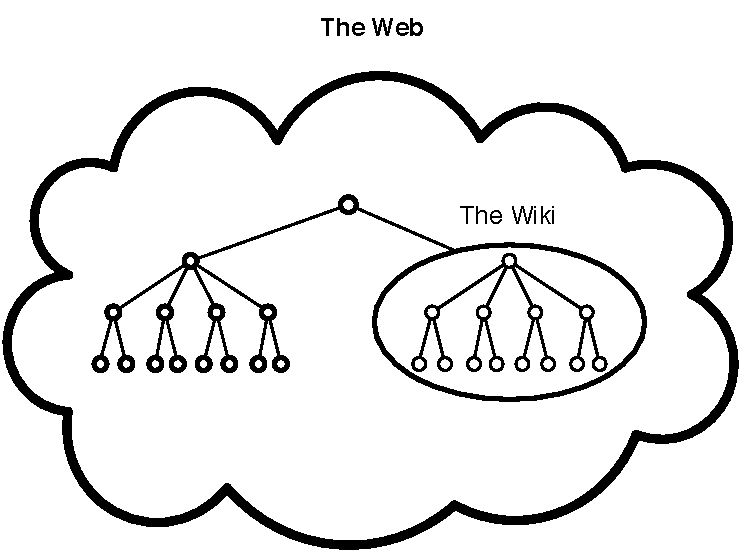
\includegraphics[width=10cm]{figs/hierarchical_structure.pdf}
\caption{The hierarchical structure of the wiki and the web.}
\label{fig:hierarchicalStructure}
\end{figure}

Note: In this report I consider the whole document set as a flat structure. Because of this I am only able find the words that are specific to a document and the words that are common for all documents.

\chapter{Implementation}
\label{cha:implementation}

The wiki uses Confluence as its platform which requires plugins to be written in Java, or at least a language that runs on the Java Virtual Machine (JVM) \cite{createPlugin}. The implementation\footnote{Implementation available at: \url{https://github.com/chrrasmussen/NTNU-Pre-Project}} is written in Clojure which runs on the JVM \cite{aboutClojure}. Because Clojure runs on the JVM, it is able to call Java-code and vice versa.

Figure~\ref{fig:trainingSystem} shows the steps involed in training the system. The implementation supports two different approaches to train the system; \textit{translate-first} and \textit{index-first}.
\begin{figure}[H]
\centering
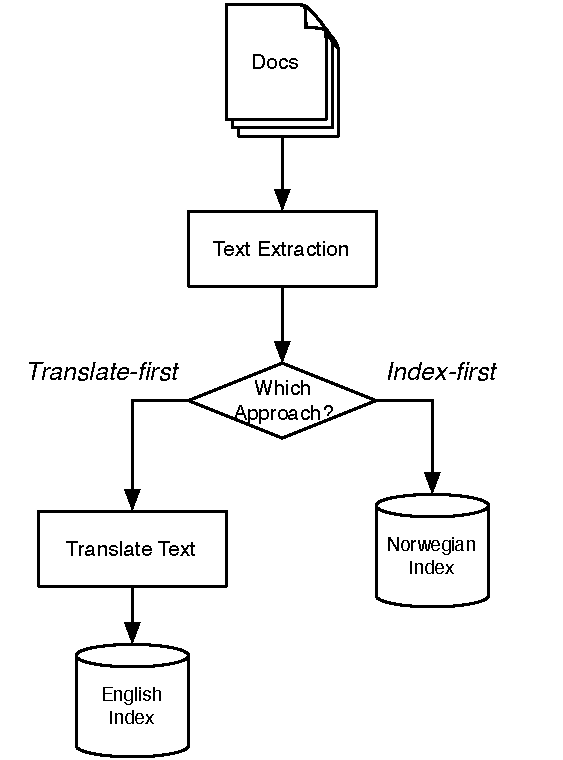
\includegraphics[height=9cm]{figs/stage1.pdf}
\caption{Stage 1 -- Training the system.}
\label{fig:trainingSystem}
\end{figure}

Figure~\ref{fig:retrieveRelatedWebPages} shows the steps involved in retrieving the related web pages for a specific document.
\begin{figure}[H]
\centering
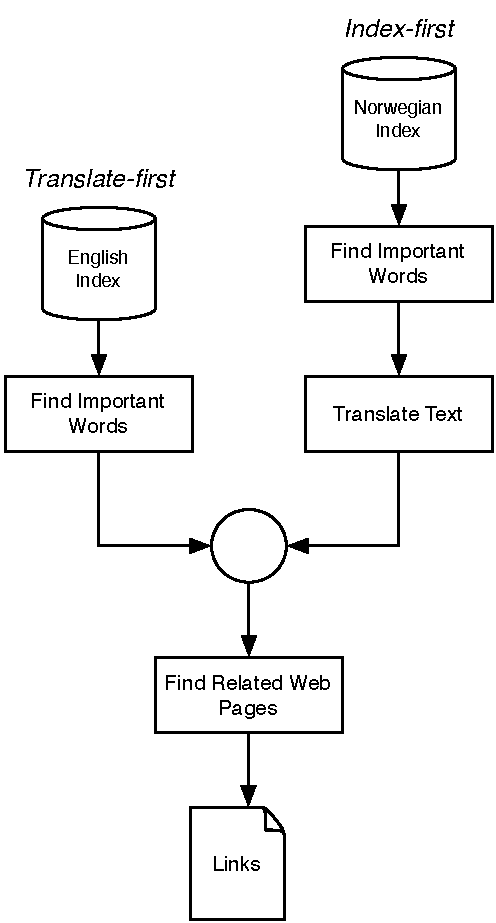
\includegraphics[height=11cm]{figs/stage2.pdf}
\caption{Stage 2 -- Retrieve related web pages.}
\label{fig:retrieveRelatedWebPages}
\end{figure}

\section{Text Extraction}
\label{sec:textExtraction}

Because the source code for the pages on the wiki are structured as XML, I must perform text extraction to get only the main content from the pages. Some pages embeds examples and charts that should be removed. These examples and charts are placed inside an element similar to: \verb|<ac:macro ac:name="code"></ac:maro>|.

My first attempt to solve the text extraction step, was to use a Java library called ``Apache Tika''. It promises to be able to ``extract metadata and structured text content from various documents using existing parser libraries'' \cite{aboutTika}.

Unfortunately, Tika turned out to be too inflexible for the task. It could only be configured to remove specific elements by name, e.g. \verb|ac:macro|. The source code for the wiki pages also include macros that should not be filtered, e.g. \verb|<ac:macro ac:name="excerpt"></ac:macro>|.

To solve the problem I turned to another Java library called ``jsoup''. This library is specialized in manipulating and extracting data from HTML documents \cite{aboutJsoup}.

\section{Translation}
\label{sec:translation}

The next step is to translate the text from Norwegian to English. The implementation uses a web service called Google Translate API \cite{aboutGoogleTranslate}. To use Google Translate you need to register a Google account.

The web service does not require any configurations.

\section{Finding Important Words}
\label{sec:findingImportantWords}

One way to find the most important words in a document is to calculate the $\tfidf$ for every word in every document. Apache Lucene is a Java library that is able to do this. However, I elected to use Apache Solr instead. Solr is a web service built on top of Lucene \cite{aboutSolr}.

Solr includes some example projects and it is easy to get up and running. This project used the bundled \verb|schema.xml| file as the starting point. To enable the calculations of $\tfidf$ for the indexed text, I added \verb|termVectors="true"| to the field named ``text''.

\section{Finding Related Web Pages}
\label{sec:searchEngine}

The last step is to find related web pages based on a query. The implementation uses a web service called Google Custom Search API \cite{aboutGoogleSearch}. To use Google Custom Search you need to register a Google account.

To use the web service you also need to configure a Custom Search Engine (CSE) for your account\footnote{Control panel to add Custom Search Engines is available at: \url{https://www.google.com/cse/}}. The CSE should be configured to search the whole web and not just some specific web pages.

\chapter{Experiments and Results}
\label{cha:experimentsAndResults}

This chapter describes the experiments that was performed in the course of this project. The results will be discussed in more details in chapter~\ref{cha:evaluationAndConclusion}.

\section{Experimental Plan}
\label{sec:experimentalPlan}

The experiments are structured to help answer the research questions (See section~\ref{sec:goalsAndResearchQuestions}).

The procedure will be as follows:
\begin{enumerate}
\item Select a few documents as sampling tests.
\item For each document:
    \begin{itemize}
    \item Get the top 5 words from the Lucene index.
    \item Apply the search queries using Google Search.
    \item Evaluate the resulting web pages.
    \end{itemize}
\end{enumerate}

For each iteration, two simultaneous experiments will be performed using separate Lucene indexes:
\begin{enumerate}
\item \textit{Translate-first} -- Documents are translated into English and then inserted into the Lucene index. Then the important words are retrieved directly from the Lucene index.
\item \textit{Index-first} -- The Norwegian documents are inserted into the Lucene index and only the important words are translated into English.
\end{enumerate}

The first itereation will be evaluated only by the author, while the second iteration will be evaluated by both the author and a committee\footnote{The committee consists of Hallvard Trætteberg.}. Each link should be assigned a rating depending on how useful the web page is from the perspective of a student. The ratings are as follows:
\begin{itemize}
\item 0 -- Not useful
\item 1 -- Somewhat useful
\item 2 -- Useful
\item 3 -- Very useful
\end{itemize}

\section{Experimental Setup}
\label{sec:experimentalSetup}

The following items are required to conduct the experiments:
\begin{itemize}
\item The source code for this project.\footnote{Implementation available at: \url{https://github.com/chrrasmussen/NTNU-Pre-Project}}
\item The documents from the wiki.
\item A Google Account to get access to Google Custom Search API and Google Translate API.
\item An installation of Apache Solr.
\end{itemize}

All experiments are based on 80 documents from the wiki, collected at 2013-11-28. About 30 of these documents are more or less empty (they are placeholders for future content). These documents are still included in the experiments but should not make any significant difference.

\section{Experimental Results -- Iteration 1}
\label{sec:experimentalResults}

To increase the likelihood for getting good results, I will choose documents that have a high average $\tfidf$. To make it easier to compare the results I will use the same five documents for every type of experiment. Thus I should choose documents that have a high average $\tfidf$ in both the \textit{translate-first} document set and the \textit{index-first} document set.

Table~\ref{tab:highestRankedDocuments-en} lists the top 10 documents from the \textit{translate-first} document set, sorted by average $\tfidf$ value.
\begin{table}[H]
\centering
\begin{tabular}{|l|c|r|c|}
\hline\hline
    Document & Avg. tf-idf & Top Word (tf-idf) & Word Count \\
\hline
    JavaFX & 16.70 & node (33.00) & 1146 \\
    Tråder med java & 6.20 & taxi (9.50) & 516 \\
    Swing & 4.84 & jframe (7.00) & 705 \\
    Tall og beregninger & 4.80 & infinity (7.00) & 747 \\
    Koding av valideringsmetoder & 4.37 & validation (13.00) & 395 \\
    Swing Timer & 4.20 & timer (10.00) & 371 \\
    Import av kode med lim inn-funksjonen & 4.00 & paste (4.00) & 305 \\
    Bruk av debuggeren i Eclipse & 3.40 & debug (5.00) & 575 \\
    Klasser i java & 3.31 & song (4.33) & 803 \\
    Anonymeklasser & 3.20 & inline (5.00) & 383 \\
\hline\hline
\end{tabular}
\caption{Top 10 documents (by avg. tf-idf) from the \textit{translate-first} document set.}
\label{tab:highestRankedDocuments-en}
\end{table}

Table~\ref{tab:highestRankedDocuments-no} lists the top 10 documents from the \textit{index-first} document set, sorted by average $\tfidf$ value.
\begin{table}[H]
\centering
\begin{tabular}{|l|c|r|c|}
\hline\hline
    Document & Avg. tf-idf & Top Word (tf-idf) & Word Count \\
\hline
    JavaFX & 12.00 & node (15.00) & 1108 \\
    Memory-eksempel versjon 1 & 4.80 & hovedprogram (5.00) & 1035 \\
    Swing & 4.80 & jpanel (6.00) & 670 \\
    Tråder med java & 4.70 & tråd (5.00) & 555 \\
    Kontrollstrukturer & 4.40 & løkker (5.00) & 701 \\
    Bruk av debuggeren i Eclipse & 4.40 & step (8.00) & 574 \\
    Swing Timer & 4.00 & timeren (8.00) & 371 \\
    Synlighetsmodifikatorer & 3.90 & ressursen (6.00) & 302 \\
    Anonymeklasser & 3.80 & anonym (6.00) & 380 \\
    Tall og beregninger & 3.80 & infinity (5.00) & 732 \\
\hline\hline
\end{tabular}
\caption{Top 10 documents (by avg. tf-idf) from the \textit{index-first} document set.}
\label{tab:highestRankedDocuments-no}
\end{table}

The documents with the highest average $\tfidf$ in both table~\ref{tab:highestRankedDocuments-en} and table~\ref{tab:highestRankedDocuments-no} are:
\begin{itemize}
\item JavaFX
\item Tråder med java
\item Swing
\item Bruk av debuggeren i Eclipse
\item Tall og beregninger
\end{itemize}

\subsection{Translate-first Experiments}
\label{subsec:experiments-en}

\subsubsection{Finding Related Web Pages for Document ``JavaFX''}
\label{subsubsec:en-javafx}

Table~\ref{tab:topWords-en-javafx} lists the top 5 words.
\begin{table}[H]
\centering
\begin{tabular}{|l|c|}
\hline\hline
    Word & tf-idf \\
\hline
    node & 33.00 \\
    scene & 20.00 \\
    nodes & 14.00 \\
    graph & 9.50 \\
    style & 7.00 \\
\hline\hline
\end{tabular}
\caption{Top 5 words from the document ``JavaFX'' in the \textit{translate-first} document set.}
\label{tab:topWords-en-javafx}
\end{table}

The search results based on the query ``node scene nodes graph style'':

\begin{enumerate}
\item
    \verb|Node (JavaFX 2.2)| \\
    \url{http://docs.oracle.com/javafx/2/api/javafx/scene/Node.html}
\item
    \verb|Scene graph - Wikipedia, the free encyclopedia| \\
    \url{http://en.wikipedia.org/wiki/Scene_graph}
\item
    \verb|javafx.scene (JavaFX 2.2)| \\
    \url{http://docs.oracle.com/javafx/2/api/javafx/scene/package-summary.html}
\item
    \verb|Chapter 3. Nodes and Groups| \\
    \url{http://techpubs.sgi.com/library/dynaweb_docs/0620/SGI_Developer/books/Inv_Mentor/sgi_html/ch03.html}
\item
    \verb|Support/Tutorials/FindingNodes – osg| \\
    \url{http://www.openscenegraph.org/projects/osg/wiki/Support/Tutorials/FindingNodes}
\end{enumerate}

Table~\ref{tab:ratings-en-javafx} shows the evaluation of each link.
\begin{table}[H]
\centering
\begin{tabular}{|l|l|}
\hline\hline
    \# & Rating (by Author) \\
\hline
    1 & 2 -- Useful \\
    2 & 1 -- Somewhat useful \\
    3 & 2 -- Useful \\
    4 & 1 -- Somewhat useful \\
    5 & 1 -- Somewhat useful \\
\hline
    Average & 1.4 \\
\hline\hline
\end{tabular}
\caption{Ratings of the links for the document ``JavaFX'' in the \textit{translate-first} document set.}
\label{tab:ratings-en-javafx}
\end{table}


%---

\subsubsection{Finding Related Web Pages for Document ``Tråder med java''}
\label{subsubsec:en-tr-der-med-java}

Table~\ref{tab:topWords-en-tr-der-med-java} lists the top 5 words.
\begin{table}[H]
\centering
\begin{tabular}{|l|c|}
\hline\hline
    Word & tf-idf \\
\hline
    taxi & 9.50 \\
    thread & 7.00 \\
    process & 5.50 \\
    driver & 5.00 \\
    client & 4.00 \\
\hline\hline
\end{tabular}
\caption{Top 5 words from the document ``Tråder med java'' in the \textit{translate-first} document set.}
\label{tab:topWords-en-tr-der-med-java}
\end{table}

The search results based on the query ``taxi thread process driver client'':

\begin{enumerate}
\item
    \verb|Shadow Market For Taxi Permits Lucrative For Some, Hardship For ...| \\
    \url{http://www.kpbs.org/news/2013/jun/10/shadow-market-taxi-permits-lucrative-some-hardship/}
\item
    \verb|Uber phone app may be shifting incentives for taxi and livery drivers ...| \\
    \url{http://www.wbez.org/news/uber-car-service-app-makes-winners-and-losers-104544}
\item
    \verb|Boston Taxis: Why Some Drivers Say Credit Cards Machines Are ...| \\
    \url{http://bostinno.streetwise.co/2013/01/28/boston-taxi-credit-card-machine-broken/}
\item
    \verb#Drivers: Uber Is Skimming Our Tips | Mother Jones# \\
    \url{http://www.motherjones.com/politics/2013/03/uber-drivers-strike-tips-wages-class-action}
\item
    \verb#HMRC targets taxi drivers...again | AccountingWEB# \\
    \url{http://www.accountingweb.co.uk/anyanswers/question/hmrc-targets-taxi-driversagain}
\end{enumerate}

Table~\ref{tab:ratings-en-tr-der-med-java} shows the evaluation of each link.
\begin{table}[H]
\centering
\begin{tabular}{|l|l|}
\hline\hline
    \# & Rating (by Author) \\
\hline
    1 & 0 -- Not useful \\
    2 & 0 -- Not useful \\
    3 & 0 -- Not useful \\
    4 & 0 -- Not useful \\
    5 & 0 -- Not useful \\
\hline
    Average & 0.0 \\
\hline\hline
\end{tabular}
\caption{Ratings of the links for the document ``Tråder med java'' in the \textit{translate-first} document set.}
\label{tab:ratings-en-tr-der-med-java}
\end{table}


%---

\subsubsection{Finding Related Web Pages for Document ``Swing''}
\label{subsubsec:en-swing}

Table~\ref{tab:topWords-en-swing} lists the top 5 words.
\begin{table}[H]
\centering
\begin{tabular}{|l|c|}
\hline\hline
    Word & tf-idf \\
\hline
    jframe & 7.00 \\
    jpanel & 6.00 \\
    component & 5.00 \\
    panel & 3.20 \\
    listener & 3.00 \\
\hline\hline
\end{tabular}
\caption{Top 5 words from the document ``Swing'' in the \textit{translate-first} document set.}
\label{tab:topWords-en-swing}
\end{table}

The search results based on the query ``jframe jpanel component panel listener'':

\begin{enumerate}
\item
    \verb|How to Write a Component Listener (The Java™ Tutorials ...| \\
    \url{http://docs.oracle.com/javase/tutorial/uiswing/events/componentlistener.html}
\item
    \verb|Java JPanel mouse listener doesn't work over its components| \\
    \url{http://stackoverflow.com/questions/9794765/java-jpanel-mouse-listener-doesnt-work-over-its-components}
\item
    \verb|Javanotes 6.0, Section 6.1 -- The Basic GUI Application| \\
    \url{http://math.hws.edu/javanotes/c6/s1.html}
\item
    \verb|java - Listening/Handling JPanel events - Stack Overflow| \\
    \url{http://stackoverflow.com/questions/10051176/listening-handling-jpanel-events}
\item
    \verb|How to Write a Component Listener| \\
    \url{http://www.math.uni-hamburg.de/doc/java/tutorial/uiswing/events/componentlistener.html}
\end{enumerate}

Table~\ref{tab:ratings-en-swing} shows the evaluation of each link.
\begin{table}[H]
\centering
\begin{tabular}{|l|l|}
\hline\hline
    \# & Rating (by Author) \\
\hline
    1 & 3 -- Very useful \\
    2 & 2 -- Useful \\
    3 & 3 -- Very useful \\
    4 & 2 -- Useful \\
    5 & 2 -- Useful \\
\hline
    Average & 2.4 \\
\hline\hline
\end{tabular}
\caption{Ratings of the links for the document ``Swing'' in the \textit{translate-first} document set.}
\label{tab:ratings-en-swing}
\end{table}


%---

\subsubsection{Finding Related Web Pages for Document ``Bruk av debuggeren i Eclipse''}
\label{subsubsec:en-bruk-av-debuggeren-i-eclipse}

Table~\ref{tab:topWords-en-bruk-av-debuggeren-i-eclipse} lists the top 5 words.
\begin{table}[H]
\centering
\begin{tabular}{|l|c|}
\hline\hline
    Word & tf-idf \\
\hline
    debug & 5.00 \\
    breakpoint & 4.00 \\
    stopped & 3.00 \\
    step & 3.00 \\
    perspective & 2.00 \\
\hline\hline
\end{tabular}
\caption{Top 5 words from the document ``Bruk av debuggeren i Eclipse'' in the \textit{translate-first} document set.}
\label{tab:topWords-en-bruk-av-debuggeren-i-eclipse}
\end{table}

The search results based on the query ``debug breakpoint stopped step perspective'':

\begin{enumerate}
\item
    \verb|Java Debugging with Eclipse - Tutorial| \\
    \url{http://www.vogella.com/articles/EclipseDebugging/article.html}
\item
    \verb|Debugger| \\
    \url{http://pydev.org/manual_adv_debugger.html}
\item
    \verb|Comp310: Debugging in Eclipse| \\
    \url{http://www.clear.rice.edu/comp310/Eclipse/debugging.html}
\item
    \verb|Effective Java Debugging with Eclipse « EclipseSource Blog| \\
    \url{http://eclipsesource.com/blogs/2013/01/08/effective-java-debugging-with-eclipse/}
\item
    \verb|About the Debug perspective| \\
    \url{http://livedocs.adobe.com/coldfusion/8/usingdebugger_5.html}
\end{enumerate}

Table~\ref{tab:ratings-en-bruk-av-debuggeren-i-eclipse} shows the evaluation of each link.
\begin{table}[H]
\centering
\begin{tabular}{|l|l|}
\hline\hline
    \# & Rating (by Author) \\
\hline
    1 & 3 -- Very useful \\
    2 & 1 -- Somewhat useful \\
    3 & 3 -- Very useful \\
    4 & 3 -- Very useful \\
    5 & 0 -- Not useful \\
\hline
    Average & 2.0 \\
\hline\hline
\end{tabular}
\caption{Ratings of the links for the document ``Bruk av debuggeren i Eclipse'' in the \textit{translate-first} document set.}
\label{tab:ratings-en-bruk-av-debuggeren-i-eclipse}
\end{table}

%---

\subsubsection{Finding Related Web Pages for Document ``Tall og beregninger''}
\label{subsubsec:en-tall-og-beregninger}

Table~\ref{tab:topWords-en-tall-og-beregninger} lists the top 5 words.
\begin{table}[H]
\centering
\begin{tabular}{|l|c|}
\hline\hline
    Word & tf-idf \\
\hline
    infinity & 7.00 \\
    range & 5.00 \\
    wrapper & 5.00 \\
    numeric & 3.50 \\
    floating & 3.50 \\
\hline\hline
\end{tabular}
\caption{Top 5 words from the document ``Tall og beregninger'' in the \textit{translate-first} document set.}
\label{tab:topWords-en-tall-og-beregninger}
\end{table}

The search results based on the query `` infinity range wrapper numeric floating'':

\begin{enumerate}
\item
    \verb|Numeric Datatypes (XML Schema)| \\
    \url{http://docstore.mik.ua/orelly/xml/schema/ch04_04.htm}
\item
    \verb|2.2 Floating point values| \\
    \url{http://www.cs.rit.edu/~ats/java-2005-2/2.2.html}
\item
    \verb|How to implement infinity in Java? - Stack Overflow| \\
    \url{http://stackoverflow.com/questions/12952024/how-to-implement-infinity-in-java}
\item
    \verb|Chapter 5. Conversions and Promotions| \\
    \url{http://docs.oracle.com/javase/specs/jls/se7/html/jls-5.html}
\item
    \verb|JavaScript Number Object| \\
    \url{http://www.w3schools.com/jsref/jsref_obj_number.asp}
\end{enumerate}

Table~\ref{tab:ratings-en-tall-og-beregninger} shows the evaluation of each link.
\begin{table}[H]
\centering
\begin{tabular}{|l|l|}
\hline\hline
    \# & Rating (by Author) \\
\hline
    1 & 1 -- Somewhat useful \\
    2 & 2 -- Useful \\
    3 & 1 -- Somewhat useful \\
    4 & 3 -- Very useful \\
    5 & 0 -- Not useful \\
\hline
    Average & 1.4 \\
\hline\hline
\end{tabular}
\caption{Ratings of the links for the document ``Tall og beregninger'' in the \textit{translate-first} document set.}
\label{tab:ratings-en-tall-og-beregninger}
\end{table}

\subsection{Index-first Experiments}
\label{subsec:experiments-no}

\subsubsection{Finding Related Web Pages for Document ``JavaFX''}
\label{subsubsec:no-javafx}

Table~\ref{tab:topWords-no-javafx} lists the top 5 words.
\begin{table}[H]
\centering
\begin{tabular}{|l|c|}
\hline\hline
    Word & tf-idf \\
\hline
    node & 15.00 \\
    scene & 14.00 \\
    noder & 11.00 \\
    graph & 11.00 \\
    id & 9.00 \\
\hline\hline
\end{tabular}
\caption{Top 5 words from the document ``JavaFX'' in the \textit{index-first} document set.}
\label{tab:topWords-no-javafx}
\end{table}

The search results based on the query ``node scene nodes graph id'':

\begin{enumerate}
\item
    \verb|Node (JavaFX 2.2)| \\
    \url{http://docs.oracle.com/javafx/2/api/javafx/scene/Node.html}
\item
    \verb|Irrlicht 3D Engine: irr::scene::ISceneManager Class Reference| \\
    \url{http://irrlicht.sourceforge.net/docu/classirr_1_1scene_1_1_i_scene_manager.html}
\item
    \verb|Ogre::SceneNode Class Reference - OGRE Documentation| \\
    \url{http://www.ogre3d.org/docs/api/html/classOgre_1_1SceneNode.html}
\item
    \verb|Irrlicht 3D Engine: Tutorial 3: Custom SceneNode| \\
    \url{http://irrlicht.sourceforge.net/docu/example003.html}
\item
    \verb|Lesson 2: The Scene Graph and Nodes| \\
    \url{http://docs.autodesk.com/3DSMAX/15/ENU/3ds-Max-SDK-Programmer-Guide/files/GUID-DCD280C9-36B4-4053-9A7F-DF03CA4F41F0.htm}
\end{enumerate}

Table~\ref{tab:ratings-no-javafx} shows the evaluation of each link.
\begin{table}[H]
\centering
\begin{tabular}{|l|l|}
\hline\hline
    \# & Rating (by Author) \\
\hline
    1 & 2 -- Useful \\
    2 & 0 -- Not useful \\
    3 & 0 -- Not useful \\
    4 & 0 -- Not useful \\
    5 & 0 -- Not useful \\
\hline
    Average & 0.4 \\
\hline\hline
\end{tabular}
\caption{Ratings of the links for the document ``JavaFX'' in the \textit{index-first} document set.}
\label{tab:ratings-no-javafx}
\end{table}


%---

\subsubsection{Finding Related Web Pages for Document ``Tråder med java''}
\label{subsubsec:no-tr-der-med-java}

Table~\ref{tab:topWords-no-tr-der-med-java} lists the top 5 words.
\begin{table}[H]
\centering
\begin{tabular}{|l|c|}
\hline\hline
    Word & tf-idf \\
\hline
    tråd & 5.00 \\
    taxisjåføren & 5.00 \\
    tråden & 5.00 \\
    taxi & 4.50 \\
    kunder & 4.00 \\
\hline\hline
\end{tabular}
\caption{Top 5 words from the document ``Tråder med java'' in the \textit{index-first} document set.}
\label{tab:topWords-no-tr-der-med-java}
\end{table}

The search results based on the query ``Thread taxi driver thread taxi customers'':

\begin{enumerate}
\item
    \verb|/vp/ - Pokémon » Thread #14770771| \\
    \url{https://archive.foolz.us/vp/thread/14770771}
\item
    \verb|I am a 26 year old NYC yellow cab driver. Ask me anything : IAmA| \\
    \url{http://www.reddit.com/r/IAmA/comments/19g9mi/i_am_a_26_year_old_nyc_yellow_cab_driver_ask_me/}
\item
    \verb|Boston should thread rightly in changing taxi system - Boston.com| \\
    \url{http://www.boston.com/2013/08/28/taxipodium/rkvcjky4As9Gl4nqXUvGmM/story.html}
\item
    \verb|Reddit Thread Of The Week: 'Scarface,' 'Taxi Driver,' And 'Harry ...| \\
    \url{http://news.moviefone.com/2012/03/30/reddit-thread-of-the-week/}
\item
    \verb|taxi driver's monopolies - WordReference Forums| \\
    \url{http://forum.wordreference.com/showthread.php?t=2741683}
\end{enumerate}

Table~\ref{tab:ratings-no-tr-der-med-java} shows the evaluation of each link.
\begin{table}[H]
\centering
\begin{tabular}{|l|l|}
\hline\hline
    \# & Rating (by Author) \\
\hline
    1 & 0 -- Not useful \\
    2 & 0 -- Not useful \\
    3 & 0 -- Not useful \\
    4 & 0 -- Not useful \\
    5 & 0 -- Not useful \\
\hline
    Average & 0.0 \\
\hline\hline
\end{tabular}
\caption{Ratings of the links for the document ``Tråder med java'' in the \textit{index-first} document set.}
\label{tab:ratings-no-tr-der-med-java}
\end{table}


%---

\subsubsection{Finding Related Web Pages for Document ``Swing''}
\label{subsubsec:no-swing}

Table~\ref{tab:topWords-no-swing} lists the top 5 words.
\begin{table}[H]
\centering
\begin{tabular}{|l|c|}
\hline\hline
    Word & tf-idf \\
\hline
    jpanel & 6.00 \\
    jframe & 6.00 \\
    lytteren & 4.00 \\
    hendelsen & 4.00 \\
    fyller & 4.00 \\
\hline\hline
\end{tabular}
\caption{Top 5 words from the document ``Swing'' in the \textit{index-first} document set.}
\label{tab:topWords-no-swing}
\end{table}

The search results based on the query ``JPanel JFrame listener event fill'':

\begin{enumerate}
\item
    \verb|java - JButtons inside JPanels, fill up the whole panel - Stack Overflow| \\
    \url{http://stackoverflow.com/questions/14550255/jbuttons-inside-jpanels-fill-up-the-whole-panel}
\item
    \verb|Javanotes 6.0, Section 6.1 -- The Basic GUI Application| \\
    \url{http://math.hws.edu/javanotes/c6/s1.html}
\item
    \verb|java - Parent JPanel - How to listen to the events generated by ...| \\
    \url{http://stackoverflow.com/questions/15753536/parent-jpanel-how-to-listen-to-the-events-generated-by-components-of-a-child-j}
\item
    \verb#Draw a filled in circle when the mouse is clicked | DaniWeb# \\
    \url{http://www.daniweb.com/software-development/java/threads/200752/draw-a-filled-in-circle-when-the-mouse-is-clicked}
\item
    \verb|java - Combining JFrame and JPanel - Stack Overflow| \\
    \url{http://stackoverflow.com/questions/15975438/combining-jframe-and-jpanel}
\end{enumerate}

Table~\ref{tab:ratings-no-swing} shows the evaluation of each link.
\begin{table}[H]
\centering
\begin{tabular}{|l|l|}
\hline\hline
    \# & Rating (by Author) \\
\hline
    1 & 1 -- Somewhat useful \\
    2 & 3 -- Very useful \\
    3 & 2 -- Useful \\
    4 & 2 -- Useful \\
    5 & 2 -- Useful \\
\hline
    Average & 2.0 \\
\hline\hline
\end{tabular}
\caption{Ratings of the links for the document ``Swing'' in the \textit{index-first} document set.}
\label{tab:ratings-no-swing}
\end{table}


%---

\subsubsection{Finding Related Web Pages for Document ``Bruk av debuggeren i Eclipse''}
\label{subsubsec:no-bruk-av-debuggeren-i-eclipse}

Table~\ref{tab:topWords-no-bruk-av-debuggeren-i-eclipse} lists the top 5 words.
\begin{table}[H]
\centering
\begin{tabular}{|l|c|}
\hline\hline
    Word & tf-idf \\
\hline
    step & 8.00 \\
    breakpoint & 4.00 \\
    fortsette & 4.00 \\
    stoppet & 3.00 \\
    breakpoints & 3.00 \\
\hline\hline
\end{tabular}
\caption{Top 5 words from the document ``Bruk av debuggeren i Eclipse'' in the \textit{index-first} document set.}
\label{tab:topWords-no-bruk-av-debuggeren-i-eclipse}
\end{table}

The search results based on the query ``step breakpoint continue stop Breakpoints'':

\begin{enumerate}
\item
    \verb|Debugging with GDB - Stopping and Continuing| \\
    \url{http://www.chemie.fu-berlin.de/chemnet/use/info/gdb/gdb_6.html}
\item
    \verb|Debugging JavaScript - Chrome DevTools — Google Developers| \\
    \url{https://developers.google.com/chrome-developer-tools/docs/javascript-debugging}
\item
    \verb|Continuing and Stepping - Debugging with GDB| \\
    \url{http://sourceware.org/gdb/onlinedocs/gdb/Continuing-and-Stepping.html}
\item
    \verb|26.2. pdb - The Python Debugger - Python v2.7.6 documentation| \\
    \url{http://docs.python.org/library/pdb.html}
\item
    \verb|Debugging Process and Features - MATLAB & Simulink| \\
    \url{http://www.mathworks.com/help/matlab/matlab_prog/debugging-process-and-features.html}
\end{enumerate}

Table~\ref{tab:ratings-no-bruk-av-debuggeren-i-eclipse} shows the evaluation of each link.
\begin{table}[H]
\centering
\begin{tabular}{|l|l|}
\hline\hline
    \# & Rating (by Author) \\
\hline
    1 & 1 -- Somewhat useful \\
    2 & 0 -- Not useful \\
    3 & 0 -- Not useful \\
    4 & 0 -- Not useful \\
    5 & 0 -- Not useful \\
\hline
    Average & 0.2 \\
\hline\hline
\end{tabular}
\caption{Ratings of the links for the document ``Bruk av debuggeren i Eclipse'' in the \textit{index-first} document set.}
\label{tab:ratings-no-bruk-av-debuggeren-i-eclipse}
\end{table}

%---

\subsubsection{Finding Related Web Pages for Document ``Tall og beregninger''}
\label{subsubsec:no-tall-og-beregninger}

Table~\ref{tab:topWords-no-tall-og-beregninger} lists the top 5 words.
\begin{table}[H]
\centering
\begin{tabular}{|l|c|}
\hline\hline
    Word & tf-idf \\
\hline
    infinity & 5.00 \\
    verdiområdet & 4.00 \\
    talltyper & 4.00 \\
    wrapper & 3.00 \\
    flyttall & 3.00 \\
\hline\hline
\end{tabular}
\caption{Top 5 words from the document ``Tall og beregninger'' in the \textit{index-first} document set.}
\label{tab:topWords-no-tall-og-beregninger}
\end{table}

The search results based on the query `` infinity range numeric types wrapper floating point'':

\begin{enumerate}
\item
    \verb|Primitive Data Types (Java in a Nutshell)| \\
    \url{http://docstore.mik.ua/orelly/java-ent/jnut/ch02_04.htm}
\item
    \verb|Chapter 5. Conversions and Promotions| \\
    \url{http://docs.oracle.com/javase/specs/jls/se7/html/jls-5.html}
\item
    \verb|Infinity - Rosetta Code| \\
    \url{http://rosettacode.org/wiki/Infinity}
\item
    \verb|Java: Floating-point| \\
    \url{http://www.leepoint.net/notes-java/data/basic_types/22floatingpoint.html}
\item
    \verb|Floating point math issues - Geos-chem| \\
    \url{http://wiki.seas.harvard.edu/geos-chem/index.php/Floating_point_math_issues}
\end{enumerate}

Table~\ref{tab:ratings-no-tall-og-beregninger} shows the evaluation of each link.
\begin{table}[H]
\centering
\begin{tabular}{|l|l|}
\hline\hline
    \# & Rating (by Author) \\
\hline
    1 & 3 -- Very useful \\
    2 & 3 -- Very useful \\
    3 & 1 -- Somewhat useful \\
    4 & 1 -- Somewhat useful \\
    5 & 0 -- Not useful \\
\hline
    Average & 1.6 \\
\hline\hline
\end{tabular}
\caption{Ratings of the links for the document ``Tall og beregninger'' in the \textit{index-first} document set.}
\label{tab:ratings-no-tall-og-beregninger}
\end{table}

\section{Experimental Results -- Iteration 2}
\label{sec:experimentalResults-2}

As described in section~\ref{sec:hierarchicalStructure}, this wiki is just any node on the web. Because of this, it could be helpful to find the words that differentiates the wiki from the rest of the web.

Because it is not feasible to create an index that contains the whole web and the wiki, I need to do an approximation. One way is to find the most common words in the current document set and filter out all the stop words.

Table~\ref{tab:top50words-en} lists the top 50 mosts commons words in \textit{translate-first} document set. The document set contains 2374 distinct words.
\begin{table}[H]
\centering
\begin{tabular}{|l|l l l l l l l l l l|}
\hline\hline
    x10 & 1 & 2 & 3 & 4 & 5 & 6 & 7 & 8 & 9 & 10 \\
\hline
    0 & and & the & to & in & of & is & as & that & a & can \\
\hline
    1 & for & be & with & are & this & it & or & an & if & code \\
\hline
    2 & not & will & one & quot & class & use & you & example & method & on \\
\hline
    3 & used & but & also & have & when & by & methods & see & more & has \\
\hline
    4 & object & what & about & java & so & which & using & classes & from & there \\
\hline\hline
\end{tabular}
\caption{Top 50 most common words in the \textit{translate-first} document set.}
\label{tab:top50words-en}
\end{table}

Table~\ref{tab:top50words-no} lists the top 50 mosts commons words in \textit{index-first} document set. The document set contains 3577 distinct words.
\begin{table}[H]
\centering
\begin{tabular}{|l|l l l l l l l l l l|}
\hline\hline
    x10 & 1 & 2 & 3 & 4 & 5 & 6 & 7 & 8 & 9 & 10 \\
\hline
    0 & er & og & som & en & i & å & for & det & til & på \\
\hline
    1 & av & kan & med & et & at & dette & har & eller & om & den \\
\hline
    2 & ikke & vil & skal & de & denne & også & være & men & brukes & ved \\
\hline
    3 & man & så & når & fra & dersom & koden & se & kode & java & slik \\
\hline
    4 & vi & over & f.eks & mer & metoder & alle & eksempel & gjøre & disse & objekter \\
\hline\hline
\end{tabular}
\caption{Top 50 most common words in the \textit{index-first} document set.}
\label{tab:top50words-no}
\end{table}

After running all the words from table~\ref{tab:top50words-en} and table~\ref{tab:top50words-no} through a filter that removes the stop words I was left with too many words. I decided to manually remove words that do not carry any meaningful information. I ended up with the word ``java'', which is very specific to document set as a whole. Thus, in the following experiments I will add the word ``java'' to the search queries.

\subsection{Translate-first Experiments}
\label{subsec:experiments-en2}

\subsubsection{Finding Related Web Pages for Document ``JavaFX''}
\label{subsubsec:no-javafx-2}

Table~\ref{tab:topWords-en-javafx-2} lists the top 5 words.
\begin{table}[H]
\centering
\begin{tabular}{|l|c|}
\hline\hline
    Word & tf-idf \\
\hline
    node & 33.00 \\
    scene & 20.00 \\
    nodes & 14.00 \\
    graph & 9.50 \\
    style & 7.00 \\
\hline\hline
\end{tabular}
\caption{Top 5 words from the document ``JavaFX'' in the \textit{translate-first} document set.}
\label{tab:topWords-en-javafx-2}
\end{table}

The search results based on the query ``java node scene nodes graph style'':

\begin{enumerate}
\item
    \verb|Node (JavaFX 2.2)| \\
    \url{http://docs.oracle.com/javafx/2/api/javafx/scene/Node.html}
\item
    \verb|javafx.scene (JavaFX 8)| \\
    \url{http://download.java.net/jdk8/jfxdocs/javafx/scene/package-summary.html}
\item
    \verb|JavaFX Architecture | JavaFX 2 Tutorials and Documentation| \\
    \url{http://docs.oracle.com/javafx/2/architecture/jfxpub-architecture.htm}
\item
    \verb|Creating Java User Interfaces with Project Scene Graph | Hello ...| \\
    \url{http://www.informit.com/articles/article.aspx?p=1323245}
\item
    \verb|JavaFX CSS Reference Guide| \\
    \url{http://docs.oracle.com/javafx/2/api/javafx/scene/doc-files/cssref.html}
\end{enumerate}

Table~\ref{tab:ratings-en-javafx-2} shows the evaluation of each link.
\begin{table}[H]
\centering
\begin{tabular}{|l|l|l|}
\hline\hline
    \# & Rating (by Author) & Rating (by Committee) \\
\hline
    1 & 2 -- Useful & 2 -- Useful \\
    2 & 2 -- Useful & 2 -- Useful \\
    3 & 3 -- Very useful & 3 -- Very useful \\
    4 & 3 -- Very useful & 2 -- Useful \\
    5 & 2 -- Useful & 2 -- Useful \\
\hline
    Average & 2.4 & 2.2 \\
\hline\hline
\end{tabular}
\caption{Ratings of the links for the document ``JavaFX'' in the \textit{translate-first} document set.}
\label{tab:ratings-en-javafx-2}
\end{table}

%---

\subsubsection{Finding Related Web Pages for Document ``Tråder med java''}
\label{subsubsec:no-tr-der-med-java-2}

Table~\ref{tab:topWords-en-tr-der-med-java-2} lists the top 5 words.
\begin{table}[H]
\centering
\begin{tabular}{|l|c|}
\hline\hline
    Word & tf-idf \\
\hline
    taxi & 9.50 \\
    thread & 7.00 \\
    process & 5.50 \\
    driver & 5.00 \\
    client & 4.00 \\
\hline\hline
\end{tabular}
\caption{Top 5 words from the document ``Tråder med java'' in the \textit{translate-first} document set.}
\label{tab:topWords-en-tr-der-med-java-2}
\end{table}

The search results based on the query ``java taxi thread process driver client'':

\begin{enumerate}
\item
    \verb|C* Summit 2013: Java and .NET Client Drivers - Cassandra ...| \\
    \url{http://www.slideshare.net/planetcassandra/cassandra-summit-data-stax-java-driver}
\item
    \verb|Observer pattern - Wikipedia, the free encyclopedia| \\
    \url{http://en.wikipedia.org/wiki/Observer_pattern}
\item
    \verb|Thread: Runtime Error 216 when using explorer.exe and Spybot| \\
    \url{http://forums.spybot.info/showthread.php?69832-Runtime-Error-216-when-using-explorer-exe-and-Spybot}
\item
    \verb|Compiled Technical Documentation| \\
    \url{https://courses.cs.washington.edu/courses/cse403/02su/www/internal/docs/TechnicalDocumentationv8.doc}
\item
    \verb|Oscar_Delta Toolbar| \\
    \url{http://forums.spybot.info/showthread.php?69789-Oscar_Delta-Toolbar}
\end{enumerate}

Table~\ref{tab:ratings-en-tr-der-med-java-2} shows the evaluation of each link.
\begin{table}[H]
\centering
\begin{tabular}{|l|l|l|}
\hline\hline
    \# & Rating (by Author) & Rating (by Committee) \\
\hline
    1 & 1 -- Somewhat useful & 0 -- Not useful \\
    2 & 0 -- Not useful & 0 -- Not useful \\
    3 & 0 -- Not useful & 0 -- Not useful \\
    4 & 0 -- Not useful & 0 -- Not useful \\
    5 & 0 -- Not useful & 0 -- Not useful \\
\hline
    Average & 0.2 & 0.0 \\
\hline\hline
\end{tabular}
\caption{Ratings of the links for the document ``Tråder med java'' in the \textit{translate-first} document set.}
\label{tab:ratings-en-tr-der-med-java-2}
\end{table}

%---

\subsubsection{Finding Related Web Pages for Document ``Swing''}
\label{subsubsec:no-swing-2}

Table~\ref{tab:topWords-en-swing-2} lists the top 5 words.
\begin{table}[H]
\centering
\begin{tabular}{|l|c|}
\hline\hline
    Word & tf-idf \\
\hline
    jframe & 7.00 \\
    jpanel & 6.00 \\
    component & 5.00 \\
    panel & 3.20 \\
    listener & 3.00 \\
\hline\hline
\end{tabular}
\caption{Top 5 words from the document ``Swing'' in the \textit{translate-first} document set.}
\label{tab:topWords-en-swing-2}
\end{table}

The search results based on the query ``java jframe jpanel component panel listener'':

\begin{enumerate}
\item
    \verb|How to Write a Component Listener (The Java™ Tutorials ...| \\
    \url{http://docs.oracle.com/javase/tutorial/uiswing/events/componentlistener.html}
\item
    \verb|Java JPanel mouse listener doesn't work over its components| \\
    \url{http://stackoverflow.com/questions/9794765/java-jpanel-mouse-listener-doesnt-work-over-its-components}
\item
    \verb|Java Swing first programs| \\
    \url{http://zetcode.com/tutorials/javaswingtutorial/firstprograms/}
\item
    \verb|java - How to resize components related to panel in swing? - Stack ...| \\
    \url{http://stackoverflow.com/questions/10784104/how-to-resize-components-related-to-panel-in-swing}
\item
    \verb|SWING ComponentListener Interface| \\
    \url{http://www.tutorialspoint.com/swing/swing_component_listener.htm}
\end{enumerate}

Table~\ref{tab:ratings-en-swing-2} shows the evaluation of each link.
\begin{table}[H]
\centering
\begin{tabular}{|l|l|l|}
\hline\hline
    \# & Rating (by Author) & Rating (by Committee) \\
\hline
    1 & 2 -- Useful & 2 -- Useful \\
    2 & 1 -- Somewhat useful & 1 -- Somewhat Useful \\
    3 & 3 -- Very useful & 2 -- Useful \\
    4 & 1 -- Somewhat useful & 1 -- Somewhat useful \\
    5 & 2 -- Useful & 1 -- Somewhat useful \\
\hline
    Average & 1.8 & 1.4 \\
\hline\hline
\end{tabular}
\caption{Ratings of the links for the document ``Swing'' in the \textit{translate-first} document set.}
\label{tab:ratings-en-swing-2}
\end{table}

%---

\subsubsection{Finding Related Web Pages for Document ``Bruk av debuggeren i Eclipse''}
\label{subsubsec:no-bruk-av-debuggeren-i-eclipse-2}

Table~\ref{tab:topWords-en-bruk-av-debuggeren-i-eclipse-2} lists the top 5 words.
\begin{table}[H]
\centering
\begin{tabular}{|l|c|}
\hline\hline
    Word & tf-idf \\
\hline
    debug & 5.00 \\
    breakpoint & 4.00 \\
    stopped & 3.00 \\
    step & 3.00 \\
    perspective & 2.00 \\
\hline\hline
\end{tabular}
\caption{Top 5 words from the document ``Bruk av debuggeren i Eclipse'' in the \textit{translate-first} document set.}
\label{tab:topWords-en-bruk-av-debuggeren-i-eclipse-2}
\end{table}

The search results based on the query ``java debug breakpoint stopped step perspective'':

\begin{enumerate}
\item
    \verb|Java Debugging with Eclipse - Tutorial| \\
    \url{http://www.vogella.com/articles/EclipseDebugging/article.html}
\item
    \verb|Effective Java Debugging with Eclipse « EclipseSource Blog| \\
    \url{http://eclipsesource.com/blogs/2013/01/08/effective-java-debugging-with-eclipse/}
\item
    \verb|Stepping through the execution of a Java program| \\
    \url{http://help.eclipse.org/indigo/topic/org.eclipse.jdt.doc.user/tasks/task-stepping.htm}
\item
    \verb|About the Debug perspective| \\
    \url{http://livedocs.adobe.com/coldfusion/8/usingdebugger_5.html}
\item
    \verb|Debugging your programs| \\
    \url{http://help.eclipse.org/juno/topic/org.eclipse.jdt.doc.user/gettingStarted/qs-13.htm}
\end{enumerate}

Table~\ref{tab:ratings-en-bruk-av-debuggeren-i-eclipse-2} shows the evaluation of each link.
\begin{table}[H]
\centering
\begin{tabular}{|l|l|l|}
\hline\hline
    \# & Rating (by Author) & Rating (by Committee) \\
\hline
    1 & 3 -- Very useful & 3 -- Very useful \\
    2 & 3 -- Very useful & 3 -- Very useful \\
    3 & 3 -- Very useful & 3 -- Very useful \\
    4 & 0 -- Not useful & 0 -- Not useful \\
    5 & 3 -- Very useful & 3 -- Very useful \\
\hline
    Average & 2.4 & 2.4 \\
\hline\hline
\end{tabular}
\caption{Ratings of the links for the document ``Bruk av debuggeren i Eclipse'' in the \textit{translate-first} document set.}
\label{tab:ratings-en-bruk-av-debuggeren-i-eclipse-2}
\end{table}

%---

\subsubsection{Finding Related Web Pages for Document ``Tall og beregninger''}
\label{subsubsec:no-tall-og-beregninger-2}

Table~\ref{tab:topWords-en-tall-og-beregninger-2} lists the top 5 words.
\begin{table}[H]
\centering
\begin{tabular}{|l|c|}
\hline\hline
    Word & tf-idf \\
\hline
    infinity & 7.00 \\
    range & 5.00 \\
    wrapper & 5.00 \\
    numeric & 3.50 \\
    floating & 3.50 \\
\hline\hline
\end{tabular}
\caption{Top 5 words from the document ``Tall og beregninger'' in the \textit{translate-first} document set.}
\label{tab:topWords-en-tall-og-beregninger-2}
\end{table}

The search results based on the query ``java infinity range wrapper numeric floating'':

\begin{enumerate}
\item
    \verb|2.2 Floating point values| \\
    \url{http://www.cs.rit.edu/~ats/java-2005-2/2.2.html}
\item
    \verb|How to implement infinity in Java? - Stack Overflow| \\
    \url{http://stackoverflow.com/questions/12952024/how-to-implement-infinity-in-java}
\item
    \verb|Chapter 5. Conversions and Promotions| \\
    \url{http://docs.oracle.com/javase/specs/jls/se7/html/jls-5.html}
\item
    \verb|Class java.lang.Double| \\
    \url{http://www.geom.uiuc.edu/~daeron/docs/apidocs/java.lang.Double.html}
\item
    \verb|Primitive Data Types (Java in a Nutshell)| \\
    \url{http://docstore.mik.ua/orelly/java-ent/jnut/ch02_04.htm}
\end{enumerate}

Table~\ref{tab:ratings-en-tall-og-beregninger-2} shows the evaluation of each link.
\begin{table}[H]
\centering
\begin{tabular}{|l|l|l|}
\hline\hline
    \# & Rating (by Author) & Rating (by Committee) \\
\hline
    1 & 2 -- Useful & 2 -- Useful \\
    2 & 1 -- Somewhat useful & 1 -- Somewhat useful \\
    3 & 2 -- Useful & 2 -- Useful \\
    4 & 2 -- Useful & 2 -- Useful \\
    5 & 3 -- Very useful & 2 -- Useful \\
\hline
    Average & 2.0 & 1.8 \\
\hline\hline
\end{tabular}
\caption{Ratings of the links for the document ``Tall og beregninger'' in the \textit{translate-first} document set.}
\label{tab:ratings-en-tall-og-beregninger-2}
\end{table}

\subsection{Index-first Experiments}
\label{subsec:experiments-no2}

\subsubsection{Finding Related Web Pages for Document ``JavaFX''}
\label{subsubsec:no-javafx-2}

Table~\ref{tab:topWords-no-javafx-2} lists the top 5 words.
\begin{table}[H]
\centering
\begin{tabular}{|l|c|}
\hline\hline
    Word & tf-idf \\
\hline
    node & 15.00 \\
    scene & 14.00 \\
    noder & 11.00 \\
    graph & 11.00 \\
    id & 9.00 \\
\hline\hline
\end{tabular}
\caption{Top 5 words from the document ``JavaFX'' in the \textit{index-first} document set.}
\label{tab:topWords-no-javafx-2}
\end{table}

The search results based on the query ``java node scene nodes graph id'':

\begin{enumerate}
\item
    \verb|Node (JavaFX 2.2)| \\
    \url{http://docs.oracle.com/javafx/2/api/javafx/scene/Node.html}
\item
    \verb|javafx.scene (JavaFX 8)| \\
    \url{http://download.java.net/jdk8/jfxdocs/javafx/scene/package-summary.html}
\item
    \verb|Parent (JavaFX 2.2)| \\
    \url{http://docs.oracle.com/javafx/2/api/javafx/scene/Parent.html}
\item
    \verb|CyberVRML97ForJava < Main < CyberGarage| \\
    \url{http://www.cybergarage.org/twiki/bin/view/Main/CyberVRML97ForJava}
\item
    \verb#Working with the JavaFX Scene Graph | JavaFX 2 Tutorials and ...# \\
    \url{http://docs.oracle.com/javafx/2/scenegraph/jfxpub-scenegraph.htm}
\end{enumerate}

Table~\ref{tab:ratings-no-javafx-2} shows the evaluation of each link.
\begin{table}[H]
\centering
\begin{tabular}{|l|l|l|}
\hline\hline
    \# & Rating (by Author) & Rating (by Committee) \\
\hline
    1 & 2 -- Useful & 2 -- Useful \\
    2 & 2 -- Useful & 2 -- Useful \\
    3 & 2 -- Useful & 2 -- Useful \\
    4 & 0 -- Not useful & 0 -- Not useful \\
    5 & 3 -- Very useful & 3 -- Very useful \\
\hline
    Average & 1.8 & 1.8 \\
\hline\hline
\end{tabular}
\caption{Ratings of the links for the document ``JavaFX'' in the \textit{index-first} document set.}
\label{tab:ratings-no-javafx-2}
\end{table}

%---

\subsubsection{Finding Related Web Pages for Document ``Tråder med java''}
\label{subsubsec:no-tr-der-med-java-2}

Table~\ref{tab:topWords-no-tr-der-med-java-2} lists the top 5 words.
\begin{table}[H]
\centering
\begin{tabular}{|l|c|}
\hline\hline
    Word & tf-idf \\
\hline
    tråd & 5.00 \\
    taxisjåføren & 5.00 \\
    tråden & 5.00 \\
    taxi & 4.50 \\
    kunder & 4.00 \\
\hline\hline
\end{tabular}
\caption{Top 5 words from the document ``Tråder med java'' in the \textit{index-first} document set.}
\label{tab:topWords-no-tr-der-med-java-2}
\end{table}

The search results based on the query ``java Thread taxi driver thread taxi customers'':

\begin{enumerate}
\item
    \verb|java - How to handle listeners if both views and models(objects ...| \\
    \url{http://stackoverflow.com/questions/11173346/}
\item
    \verb|Tests Don't Run · Issue #1 · clojure-cookbook/browser-testing · GitHub| \\
    \url{https://github.com/clojure-cookbook/browser-testing/issues/1}
\item
    \verb|Taxi Drivers - Pokémon X & Y Forum - Neoseeker Forums| \\
    \url{http://www.neoseeker.com/forums/60943/t1914668-taxi-drivers/}
\item
    \verb|Stupid cab drivers around metropolitan Phoenix. (Tempe ...| \\
    \url{http://www.city-data.com/forum/phoenix-area/947792-stupid-cab-drivers-around-metropolitan-phoenix.html}
\item
    \verb|Russian app-based taxi startup Wheely takes aim at London's ...| \\
    \url{http://www.computing.co.uk/ctg/news/2273632/russian-appbased-taxi-startup-wheely-takes-aim-at-londons-addison-lee}
\end{enumerate}

Table~\ref{tab:ratings-no-tr-der-med-java-2} shows the evaluation of each link.
\begin{table}[H]
\centering
\begin{tabular}{|l|l|l|}
\hline\hline
    \# & Rating (by Author) & Rating (by Committee) \\
\hline
    1 & 1 -- Somewhat useful & 1 -- Somewhat useful \\
    2 & 0 -- Not useful & 0 -- Not useful \\
    3 & 0 -- Not useful & 0 -- Not useful \\
    4 & 0 -- Not useful & 0 -- Not useful \\
    5 & 0 -- Not useful & 0 -- Not useful \\
\hline
    Average & 0.2 & 0.2 \\
\hline\hline
\end{tabular}
\caption{Ratings of the links for the document ``Tråder med java'' in the \textit{index-first} document set.}
\label{tab:ratings-no-tr-der-med-java-2}
\end{table}

%---

\subsubsection{Finding Related Web Pages for Document ``Swing''}
\label{subsubsec:no-swing-2}

Table~\ref{tab:topWords-no-swing-2} lists the top 5 words.
\begin{table}[H]
\centering
\begin{tabular}{|l|c|}
\hline\hline
    Word & tf-idf \\
\hline
    jpanel & 6.00 \\
    jframe & 6.00 \\
    lytteren & 4.00 \\
    hendelsen & 4.00 \\
    fyller & 4.00 \\
\hline\hline
\end{tabular}
\caption{Top 5 words from the document ``Swing'' in the \textit{index-first} document set.}
\label{tab:topWords-no-swing-2}
\end{table}

The search results based on the query ``java JPanel JFrame listener event fill'':

\begin{enumerate}
\item
    \verb|java - JButtons inside JPanels, fill up the whole panel - Stack Overflow| \\
    \url{http://stackoverflow.com/questions/14550255/jbuttons-inside-jpanels-fill-up-the-whole-panel}
\item
    \verb|Javanotes 6.0, Section 6.1 -- The Basic GUI Application| \\
    \url{http://math.hws.edu/javanotes/c6/s1.html}
\item
    \verb|java - JTable update after row selection - Stack Overflow| \\
    \url{http://stackoverflow.com/questions/20443764/jtable-update-after-row-selection}
\item
    \verb|JAVA SWING GUI TUTORIAL| \\
    \url{http://cs.nyu.edu/~yap/classes/visual/03s/lect/l7/}
\item
    \verb|ChartPanel (JFreeChart Class Library (version 1.0.17))| \\
    \url{http://www.jfree.org/jfreechart/api/javadoc/org/jfree/chart/ChartPanel.html}
\end{enumerate}

Table~\ref{tab:ratings-no-swing-2} shows the evaluation of each link.
\begin{table}[H]
\centering
\begin{tabular}{|l|l|l|}
\hline\hline
    \# & Rating (by Author) & Rating (by Committee) \\
\hline
    1 & 2 -- Useful & 1 -- Somewhat useful \\
    2 & 3 -- Very useful & 3 -- Very useful \\
    3 & 1 -- Somewhat useful & 0 -- Not useful \\
    4 & 3 -- Very useful & 3 -- Very useful \\
    5 & 1 -- Somewhat useful & 0 -- Not useful \\
\hline
    Average & 2.0 & 1.4 \\
\hline\hline
\end{tabular}
\caption{Ratings of the links for the document ``Swing'' in the \textit{index-first} document set.}
\label{tab:ratings-no-swing-2}
\end{table}

%---

\subsubsection{Finding Related Web Pages for Document ``Bruk av debuggeren i Eclipse''}
\label{subsubsec:no-bruk-av-debuggeren-i-eclipse-2}

Table~\ref{tab:topWords-no-bruk-av-debuggeren-i-eclipse-2} lists the top 5 words.
\begin{table}[H]
\centering
\begin{tabular}{|l|c|}
\hline\hline
    Word & tf-idf \\
\hline
    step & 8.00 \\
    breakpoint & 4.00 \\
    fortsette & 4.00 \\
    stoppet & 3.00 \\
    breakpoints & 3.00 \\
\hline\hline
\end{tabular}
\caption{Top 5 words from the document ``Bruk av debuggeren i Eclipse'' in the \textit{index-first} document set.}
\label{tab:topWords-no-bruk-av-debuggeren-i-eclipse-2}
\end{table}

The search results based on the query ``java step breakpoint continue stop Breakpoints'':

\begin{enumerate}
\item
    \verb|Debugging JavaScript - Chrome DevTools — Google Developers| \\
    \url{https://developers.google.com/chrome-developer-tools/docs/javascript-debugging}
\item
    \verb|Debugging Java programs with BlueJ| \\
    \url{http://www.mathcs.emory.edu/~cheung/Courses/170/Syllabus/02/BlueJ/BlueJ3.html}
\item
    \verb|Debugging with GDB - Stopping and Continuing| \\
    \url{http://www.chemie.fu-berlin.de/chemnet/use/info/gdb/gdb_6.html}
\item
    \verb|Java Debugging with Eclipse - Tutorial| \\
    \url{http://www.vogella.com/articles/EclipseDebugging/article.html}
\item
    \verb|C H A P T E R    6 - Setting Breakpoints and Traces| \\
    \url{http://docs.oracle.com/cd/E19422-01/819-3683/breakpnt.html}
\end{enumerate}

Table~\ref{tab:ratings-no-bruk-av-debuggeren-i-eclipse-2} shows the evaluation of each link.
\begin{table}[H]
\centering
\begin{tabular}{|l|l|l|}
\hline\hline
    \# & Rating (by Author) & Rating (by Committee) \\
\hline
    1 & 0 -- Not useful & 0 -- Not useful \\
    2 & 2 -- Useful & 0 -- Not useful \\
    3 & 0 -- Not useful & 0 -- Not useful \\
    4 & 3 -- Very useful & 3 -- Very useful \\
    5 & 3 -- Very useful & 0 -- Not useful \\
\hline
    Average & 1.6 & 0.6 \\
\hline\hline
\end{tabular}
\caption{Ratings of the links for the document ``Bruk av debuggeren i Eclipse'' in the \textit{index-first} document set.}
\label{tab:ratings-no-bruk-av-debuggeren-i-eclipse-2}
\end{table}

%---

\subsubsection{Finding Related Web Pages for Document ``Tall og beregninger''}
\label{subsubsec:no-tall-og-beregninger-2}

Table~\ref{tab:topWords-no-tall-og-beregninger-2} lists the top 5 words.
\begin{table}[H]
\centering
\begin{tabular}{|l|c|}
\hline\hline
    Word & tf-idf \\
\hline
    infinity & 5.00 \\
    verdiområdet & 4.00 \\
    talltyper & 4.00 \\
    wrapper & 3.00 \\
    flyttall & 3.00 \\
\hline\hline
\end{tabular}
\caption{Top 5 words from the document ``Tall og beregninger'' in the \textit{index-first} document set.}
\label{tab:topWords-no-tall-og-beregninger-2}
\end{table}

The search results based on the query ``java infinity range numeric types wrapper floating point'':

\begin{enumerate}
\item
    \verb|Primitive Data Types (Java in a Nutshell)| \\
    \url{http://docstore.mik.ua/orelly/java-ent/jnut/ch02_04.htm}
\item
    \verb|Chapter 5. Conversions and Promotions| \\
    \url{http://docs.oracle.com/javase/specs/jls/se7/html/jls-5.html}
\item
    \verb|Java: Floating-point| \\
    \url{http://www.leepoint.net/notes-java/data/basic_types/22floatingpoint.html}
\item
    \verb|How to implement infinity in Java? - Stack Overflow| \\
    \url{http://stackoverflow.com/questions/12952024/how-to-implement-infinity-in-java}
\item
    \verb|2.2 Floating point values| \\
    \url{http://www.cs.rit.edu/~ats/java-2005-2/2.2.html}
\end{enumerate}

Table~\ref{tab:ratings-no-tall-og-beregninger-2} shows the evaluation of each link.
\begin{table}[H]
\centering
\begin{tabular}{|l|l|l|}
\hline\hline
    \# & Rating (by Author) & Rating (by Committee) \\
\hline
    1 & 3 -- Very useful & 2 -- Useful \\
    2 & 3 -- Very useful & 2 -- Useful \\
    3 & 1 -- Somewhat useful & 1 -- Somewhat useful \\
    4 & 1 -- Somewhat useful & 1 -- Somewhat useful \\
    5 & 2 -- Useful & 2 -- Useful \\
\hline
    Average & 2.0 & 1.6 \\
\hline\hline
\end{tabular}
\caption{Ratings of the links for the document ``Tall og beregninger'' in the \textit{index-first} document set.}
\label{tab:ratings-no-tall-og-beregninger-2}
\end{table}

\chapter{Evaluation and Conclusion}
\label{cha:evaluationAndConclusion}

This chapter concludes the report by evaluating and discussing the results from chapter~\ref{cha:experimentsAndResults}.

\section{Evaluation}
\label{sec:evaluation}

Table~\ref{tab:averageResults} lists the average rating of each experiment.
\begin{table}[H]
\centering
\begin{tabular}{|l|c|c|c|c|c|c|}
\hline\hline
     & \multicolumn{2}{|c|}{Iteration 1} & \multicolumn{2}{|c|}{Iteration 2} \\
\cline{2-5}
    Document & Translate-first & Index-first & Translate-first & Index-first \\
\hline
    JavaFX                          & 1.4 & 0.4 & 2.4 (2.2) & 1.8 (1.8) \\
    Tråder med java                 & 0.0 & 0.0 & 0.2 (0.0) & 0.2 (0.2) \\
    Swing                           & 2.4 & 2.0 & 1.8 (1.4) & 2.0 (1.4) \\
    Bruk av debuggeren i Eclipse    & 2.0 & 0.2 & 2.4 (2.4) & 1.6 (0.6) \\
    Tall og beregninger             & 1.4 & 1.6 & 2.0 (1.8) & 2.0 (1.6) \\
\hline\hline
\end{tabular}
\caption{The average rating of each experiment (results in parenthesis are evaluated by committee).}
\label{tab:averageResults}
\end{table}

\subsubsection{Translate-first vs. Index-first}

By comparing the results from the \textit{translate-first} experiments and the results from the \textit{index-first} experiments, we can see that the \textit{translate-first} approach gives the highest average rating in most cases.

\subsubsection{Iteration 1 vs. Iteration 2}

By comparing the results between iteration 1 and iteration 2 we can see that the addition of the word ``java'' in the search query gives a higher average rating in most cases.

\subsubsection{Anomalous Results}

In table~\ref{tab:averageResults} there is one document that stands out from the rest; the document ``Tråder med java''. It seems like none of the resulting web pages were useful from the perspective of a student.

By looking at the results from the experiments (from section~\ref{sec:experimentalResults} and section~\ref{sec:experimentalResults-2}) one common feature among the web pages is that they are related to the word ``taxi'', in the context of the profession taxi driver. This might indicate that Google Search weights the word ``taxi'' higher than the others words. Table~\ref{tab:searchQueries-tr-der-med-java} lists the search queries used in the different experiments.
\begin{table}[H]
\centering
\begin{tabular}{|l|l|}
\hline\hline
    Experiment & Search Query \\
\hline
    Iteration 1, \nameref{subsec:experiments-en} & taxi thread process driver client \\
    Iteration 1, \nameref{subsec:experiments-no} & Thread taxi driver thread taxi customers \\
    Iteration 2, \nameref{subsec:experiments-en2} & java taxi thread process driver client \\
    Iteration 2, \nameref{subsec:experiments-no2} & java Thread taxi driver thread taxi customers \\
\hline\hline
\end{tabular}
\caption{The search queries used to find related web pages for the document ``Tråder med java''.}
\label{tab:searchQueries-tr-der-med-java}
\end{table}

But why is the word ``taxi'' in the search query in the first place? By looking at the content of the document ``Tråder med java'' (See attachment~\ref{att:confluence-tr-der-med-java}) we can see that the word ``taxi'' occurs multiple times in an example which explains threads in Java.

\section{Discussion}
\label{sec:discussion}

Because the documents that were selected were the ones with the highest average $\tfidf$, this approach might not work as well for documents with a lower average $\tfidf$.

\subsubsection{Translate-first vs. Index-first}

The results indicate that the \textit{translate-first} is a better approach than \textit{index-first} approach. There might be several reasons for this:
\begin{itemize}
\item In the case of \textit{translate-first} approach, a complete document is translated at the time, which gives the translator the full context of all the words. This might give a more accurate translation of all the words.
\item The documents in the wiki does not always use the Norwegian translation of the terminology in computer science. E.g. both ``tråd'' and ``thread'' are added to the index. Because of this, the \textit{index-first} index ends up with a lot more words (3577 distinct words) than the \textit{translate-first} index (2374 distinct words).
\end{itemize}

\subsubsection{Iteration 1 vs. Iteration 2}

The results indicate that the addition of ``java'' improves the results. The main reason for this is probably that the search query is more specific (includes more keywords). The keyword ``java'' is a word that describe the whole document set.

To further improve the algorithm, keywords that only characterize a subset of the document set could be used. For example, if the document is structured below the Eclipse-category, the word ``Eclipse'' could be a a keyword in the search query.

\subsubsection{Anomalous Results}

As described in section~\ref{sec:evaluation}, the document ``Tråder med java'' did not yield any related web pages. This was mainly caused by a word (``taxi'') that was accidentally picked as an important word for that document. One way to fix this is to tag a portion of the document as an example, or more fine-grained, tag specific words or phrases, e.g. ``Taxi Trondheim AS'', as entities. This could be done manually or automatically using a technique called Named-Entity Recognition (NER) \cite{introToIR}. By tagging the content it is easier to extract only the desired text.

\section{Conclusion}
\label{sec:conclusion}

The \textit{translate-first} approach with additional keywords (which characterize the document set or a subset of it) does show some potential. However, this report has focused on the best-case scenario, and the approach might not work as well for all documents.

\section{Future Work}
\label{sec:futureWork}

As seen in section~\ref{sec:discussion}, there are a number of changes that might improve the results in this project:
\begin{itemize}
\item Add more keywords to the search query -- This will give more specific results but at the risk that it yields no results.
\item Use keywords that are specific to a only subset of the doument set -- This will for example add ``Eclipse'' to the search query for the documents that are located below the Eclipse-category.
\item Boost fields in the Lucene index -- This will give extra weight to certain words, e.g. the title of the documents.
\item Evaluate relevancy of the search results -- This will filter irrelevant links before the user even sees them.
\item Add Named-Entity Recognition -- This will give a higher control of what content that will be added to the Lucene index.
\end{itemize}

Finally, the implementation could be turned into a working plugin for Confluence. This plugin can either embed the links automatically or suggest links to the author who must approve them.

\backmatter

\addcontentsline{toc}{chapter}{Bibliography}
\bibliography{bibtex/bibliography}

\chapter{Attachments}
\label{cha:attachments}

\begin{enumerate}
\item\label{att:confluence-tr-der-med-java} Confluence Printout -- ``Tråder med java''
\end{enumerate}

\cleardoublepage

\end{document}